

Em relação ao método KMeans para agrupar as estrelas de acordo com suas características, é necessário escolher um estado alatório (\verb|random_state = |) para aplicação do KMeans, pois caso contrário, a análise não torna-se reprodutível, dado que para cada estado aleatório escolhido pelo próprio KMeans, a quantidade ótima de \textit{clusters} vai sempre mudar, prejudicando a análise. Portanto, podemos escolher um \verb|random_state = 2|\footnote{A escolha do \texttt{random\_state = 2} é feita com base na quantidade de tipos existentes na tabela \texttt{Categorias.csv}, pois a análise, \textit{a posteriori}, indica que o número ideal de \textit{clusters} é igual a 6. Foi estudada a possibilidade de diminuir a tolerância do KMeans (que por padrão é \texttt{0.0001}) para evitar que os gráficos se alterem a cada compilação, porém mesmo diminuindo até $10^{-20}$, sempre ocorria uma mudança no fator de silhueta, influenciando diretamente na quantidade de \textit{clusters} e portanto na análise.} na implementação do KMeans. Construímos então o fato de silhueta importando o \verb|KMeans| da biblioteca \verb|sklearn.cluster|.
\begin{longlisting}
    \begin{minted}{py}
        from sklearn.cluster import KMeans
        
        silKMeans = []
        for n in range(2, 11):
            kmeans = KMeans(n_clusters=n, random_state=2).fit(scaledNumdS)
            labels = kmeans.fit_predict(scaledNumdS)
            silKMeans.append(silhouette_score(scaledNumdS, labels))
        
        plt.plot(range(2,11), silKMeans, marker='o')
        plt.xlabel('Número de Clusters')
        plt.ylabel('Fator de Silhueta')
        plt.show()
    \end{minted}
\end{longlisting}
\begin{figure}[H]
    \centering
    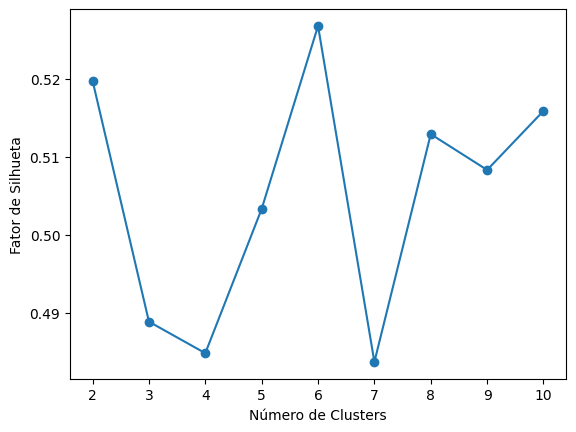
\includegraphics[width=0.5\linewidth]{figures/KMeansSilhouette.png}
\end{figure}

Com isso, somos capazes de formar os \textit{clusters} definindo uma variável que armazena o valor máximo do fator de silhueta e aplicando \verb|n_clusters| igual a este valor.
\begin{longlisting}
    \begin{minted}{py}
        bestNumberClustersKMeans = list(range(2,11))[np.argmax(silKMeans)]

        kmeans = KMeans(n_clusters=bestNumberClustersKMeans).fit(scaledNumdS)
        categoriasKMeans = kmeans.labels_
        
        plt.figure(figsize=(15,10))
        for i, (xVar, yVar) in enumerate([('Temperature', 'L'), ('R','A_M'), ('Temperature','R'), ('L','A_M'), ('Temperature', 'A_M'), ('R','L')], 1):
            plt.subplot(2,3,i)
            plt.scatter(scaledNumdS[xVar], scaledNumdS[yVar], c=categoriasKMeans, cmap='inferno')
            plt.xlabel(xVar)
            plt.ylabel(yVar)
    \end{minted}
\end{longlisting}
\begin{figure}[H]
    \centering
    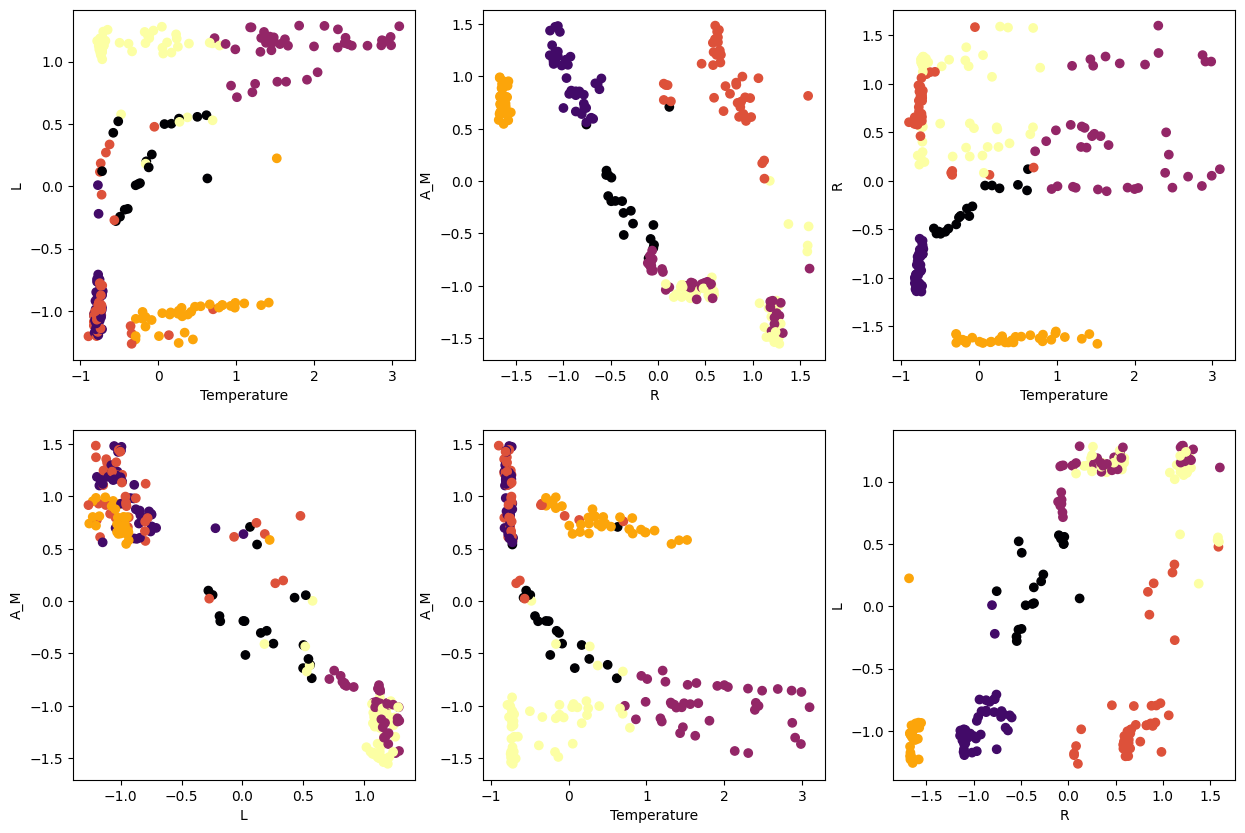
\includegraphics[width=1\linewidth]{figures/KMeans.png}
\end{figure}
